\documentclass[conference]{IEEEtran}

\usepackage{amsmath}
\usepackage{amssymb}
\usepackage{blindtext}
\usepackage{booktabs}
\usepackage{caption}
\usepackage{graphicx}
\usepackage[utf8]{inputenc}
\usepackage{multirow}
\usepackage[group-separator={,}]{siunitx}
\usepackage[x11names, rgb, dvipsnames]{xcolor}
\usepackage{xfrac}
\usepackage[perpage]{footmisc}
\usepackage[hidelinks=true]{hyperref}
\usepackage{microtype}
\usepackage[capitalize, nameinlink, noabbrev]{cleveref}
\usepackage{subcaption}

\usepackage{tikz}
\usetikzlibrary{shapes}
\usetikzlibrary{arrows}

\bibliographystyle{alpha}

\DeclareMathOperator{\ypred}{y_{pred}}
\DeclareMathOperator{\ytrue}{y_{true}}

\DeclareMathOperator{\rank}{rank}
\DeclareMathOperator{\cov}{cov}

\DeclareMathOperator{\TP}{TP}
\DeclareMathOperator{\TN}{TN}
\DeclareMathOperator{\FP}{FP}
\DeclareMathOperator{\FN}{FN}
\DeclareMathOperator{\FPR}{FPR}
\DeclareMathOperator{\AUC}{AUC}
\DeclareMathOperator{\TNR}{TNR}
\DeclareMathOperator{\TNA}{TNA}
\DeclareMathOperator{\TPA}{TPA}
\DeclareMathOperator{\TPR}{TPR}

\DeclareMathOperator{\Precision}{Precision}
\DeclareMathOperator{\Recall}{Recall}
\DeclareMathOperator{\InvPrecision}{Inverse\ Precision}
\DeclareMathOperator{\InvRecall}{Inverse\ Recall}
\DeclareMathOperator{\Accuracy}{Accuracy}

\DeclareMathOperator{\calls}{calls}
\DeclareMathOperator{\etime}{time}
\DeclareMathOperator{\sms}{sms}
\DeclareMathOperator{\contacts}{contacts}

\DeclareMathOperator{\ein}{in}
\DeclareMathOperator{\out}{out}

\DeclareMathOperator{\low}{low}
\DeclareMathOperator{\high}{high}

\DeclareMathOperator{\train}{train}
\DeclareMathOperator{\test}{test}

\DeclareMathOperator{\Betainc}{\Beta_{\operatorname{inc}}}

\DeclareMathOperator{\incalls}{incalls}
\DeclareMathOperator{\outcalls}{outcalls}
\DeclareMathOperator{\insms}{insms}
\DeclareMathOperator{\outsms}{insms}
\DeclareMathOperator{\intime}{outtime}
\DeclareMathOperator{\outtime}{outtime}
\DeclareMathOperator{\incontacts}{incontacts}
\DeclareMathOperator{\outcontacts}{outcontacts}

\DeclareMathOperator{\incallslow}{incallslow}
\DeclareMathOperator{\outcallslow}{outcallslow}
\DeclareMathOperator{\insmslow}{insmslow}
\DeclareMathOperator{\outsmslow}{insmslow}
\DeclareMathOperator{\intimelow}{outtimelow}
\DeclareMathOperator{\outtimelow}{outtimelow}
\DeclareMathOperator{\incontactslow}{incontactslow}
\DeclareMathOperator{\outcontactslow}{outcontactslow}

\DeclareMathOperator{\incallshigh}{incallshigh}
\DeclareMathOperator{\outcallshigh}{outcallshigh}
\DeclareMathOperator{\insmshigh}{insmshigh}
\DeclareMathOperator{\outsmshigh}{insmshigh}
\DeclareMathOperator{\intimehigh}{outtimehigh}
\DeclareMathOperator{\outtimehigh}{outtimehigh}
\DeclareMathOperator{\incontactshigh}{incontactshigh}
\DeclareMathOperator{\outcontactshigh}{outcontactshigh}

\DeclareMathOperator{\neigh}{Neigh}

\DeclareMathOperator{\dir}{dir}
\DeclareMathOperator{\cat}{cat}

\DeclareMathOperator{\ego}{ego}

\DeclareMathOperator{\logit}{logit}

\DeclareMathOperator{\Betadist}{Beta}
\DeclareMathOperator{\Binomial}{Bin}


\newcommand{\todo}[1]{\textbf{\color{red} TODO:\@ #1}}
\newcommand{\maybe}[1]{\footnote{\color{red} #1}}

\newcommand{\NA}{---}
\newcommand{\ct}[1]{\multicolumn{1}{c}{#1}}

\newcommand{\noimage}{%
  \setlength{\fboxsep}{-\fboxrule}
  \fbox{\phantom{\rule{\columnwidth}{100pt}}}
}
\newcommand{\includegraphicsmaybe}[1]{\IfFileExists{#1}{\includegraphics[width=\columnwidth, height=.24\textheight, keepaspectratio]{#1}}{\noimage}}

\renewcommand{\thefootnote}{\fnsymbol{footnote}}
\captionsetup[table]{skip = 2ex}

\title{Comparison of Feature Extraction Methods and Predictors for Income Inference}

\author{%
\IEEEauthorblockN{%
	Martin Fixman\IEEEauthorrefmark{1},
	Martin Minnoni\IEEEauthorrefmark{2},
	Carlos Sarraute\IEEEauthorrefmark{2}
}
\IEEEauthorblockA{\IEEEauthorrefmark{1}Universidad de Buenos Aires, Argentina}
\IEEEauthorblockA{\IEEEauthorrefmark{2}Grandata Labs, 550 15th Street, San Francisco, CA, USA}
\IEEEauthorblockA{Email: martinfixman@gmail.com, \{martin, charles\}@grandata.com}
}

\begin{document}
\maketitle

\begin{abstract}
Obtaining and processing demographical and sociological data have been some of the most important processes for understanding population-wide phenomena since at least 17th century~\cite{friendly2006}, and finding simple and intuitive ways of visualizing them has a big impact in our ways of understanding the data~\cite{minard1844,snow1855}. Common ways of obtaining useful qualitative data on socioeconomic stratification usually involved archival research or social surveys~\cite{bulmer1977}; however those methods can't present data that's at the same time exact, up to date, and that applies to a large population without having to rely on statistical methods.

Telecommunication operators (``telcos'') have access to a wealth of information about their users' communications and habits~\cite{huurdeman2003}, but the ability to store and process that data has taken large strides in the last few years thanks to new and more powerful computers and data mining techniques. The same can be said for sociological and economic information owned by banks and credit cards, and the relation between these two data sources.

Large scale data mining of data from the telecommunications industry is a relatively new area that's been so far mostly used for internal applications~\cite{han2002emerging}, but the gigantic wealth of real-time sociological data has been of interest for academic purposes related to sociology. This thesis builds on methods used by Óskardottir et.\ al.~\cite{oskardottir2016} and Singh et.\ al~\cite{singh2013predicting}, along with a large dataset of information for a certain telco and a large bank to find that the income distribution of the users follows closely (but not exactly) the income distribution of the whole population.

There's a strong homophily between the incomes of contacts in the telco, which along with the uneven distribution of wealth in the population is leveraged to create a methodology, grounded in Bayesian statistics, to infer socioeconomic level of a large subset of users in the network without banking information which is very accurate at $\AUC = 0.746$. The Bayesian method is later compared to several other methods based on supervised machine learning to prove that, even though it uses less input information, it's a better predictor of social features in this particular kind of network.

% In this work, we examine the socio-economic correlations present among users in a mobile phone network. First, we find that the distribution of income for a subset of users, for which we have income information given by a large bank, follows closely, but not exactly, the income distribution for the whole population. We also show the existence of a strong socio-economic homophily in the mobile phone network, where users linked in the network are more likely to have similar income. The main contribution of this work is that we leverage this homophily in order to propose a methodology, based on Bayesian statistics, to infer the socio-economic status for a large subset of users in the network (for which we have no banking information). With our proposed algorithm, we create an estimator for two categories (low and high income) which significantly outperforms both a simpler method based on a frequentist approach and several common \emph{Machine Learning} methods.

\end{abstract}

% !TEX root = tesis.tex

\chapter{Introduction}

% MOTIVATION
\section{Motivation of the Thesis}

In recent years, we have witnessed an exponential growth in the capacity to gather, store and manipulate massive amounts of data across a broad spectrum of disciplines: in astrophysics our capacity to gather and analyze massive datasets from astronomical observations has significantly transformed our capacity to model the dynamics of our cosmos; in sociology our capacity to track and study traits from individuals within a population of millions is allowing us to create social models at multiple scales, tracking individual and collective behavior both in space and time, with a granularity not even imagined twenty years ago.

In particular, mobile phone datasets provide a very rich view into the social interactions and the physical movements of large segments of a population. The voice calls and text messages exchanged between people, together with the call locations (recorded through cell tower usages), allow us to construct a rich social graph which can give us interesting insights on the users' social fabric, detailing not only particular social relationships and traits, but also regular patterns of behavior both in space and time, such as their daily and weekly mobility patterns~\cite{gonzalez2008understanding,ponieman2013human,sarraute2015city}.

Demographic factors play an important role in the constitution and preservation of social links. In particular concerning their age, individuals have a tendency to
establish links with others of similar age. This phenomenon is called age homophily~\cite{mcpherson2001birds}, and has been verified in mobile phone communications graph~\cite{blumenstock2010mobile,sarraute2014} as well as the Facebook graph~\cite{ugander2011anatomy}.


% PREVIOUS WORK ON THIS PROBLEM

Economic factors are also believed to have a determining role in both the social network's structure and dynamics. However, there are still very few large-scale quantitative analyses on the interplay between economic status of individuals and their social network. In~\cite{leo2015socioeconomic}, the authors analyze the correlations between mobile phone data and banking transaction information, revealing the existence of social stratification. They also show the presence of socioeconomic homophily among the networks participants using users' income, purchasing power and debt as indicators.
The authors of \cite{Luo2017inferring} studied the correlation between the position of a node in a mobile phone communications graph and its socio-economic status. They showed that the position and topological attributes in the graph can be used to generate inferences of the users' financial status.
In particular the study \cite{Luo2017inferring} shows the value of the Collective Influence~\cite{morone2015influence} as a topological attribute for the prediction of individual financial status.


% SUMMARY OF THE NEW APPROACH
\section{Summary of our Approach}

In this work, we leverage the socioeconomic homophily present in the cellular phone network to generate inferences of socioeconomic status in the communication graph. To this aim we will use the following data sources: (i) the Call Detail Records (CDRs) from the operator allow us to construct a social graph and to establish social affinities among users; (ii) banking reported income for a subset of their clients obtained from a large bank data source. We then construct an inferential algorithm that allows us to predict the socioeconomic status of users close to those for which we have banking information. To our knowledge, this is the first time both mobile phone and banking information has been integrated in this way to make inferences based on a social telecommunication graph.
Part of this work was published in~\cite{Fixman2016bayesian}.

The work done on this thesis is based the hypotheses that there is a significant level of homophily between a person's socioeconomic level and the one from its contacts (\cref{subsec:income_homophily}), and that using this correlation we can infer the first from the second (\cref{subsec:prediction_algorithm}).
At the same time, this thesis presents several ``conventional'' Machine Learning algorithms (\cref{sec:comparison}) along with an inference algorithm based in Bayesian Inference which works thanks to the correlation hypothesis (\cref{sec:inference_methodology}). This extra information should give this algorithm better results than the conventional ones.

Multiple strategies can be used to generate network features based on the CDRs. For instance, in \cite{oskarsdottir2016} the authors evaluate different collective inference methods applied to the churn prediction problem. Furthermore, the work \cite{oskarsdottir2017social} studies the impact of the social graph definition on the performance of the prediction methods. This motives the second part of the thesis, where we perform a comparative study of methods to generate network features for the nodes in the communication graph, and evaluate their impact on the inference of the income. We also compare the effectiveness of machine learning methods such as Logistic Regression and Random Forest on the different feature sets.

\todo{Add a summary of results}

\section{Organisation of the Thesis}

The remainder of the thesis is organized as follows.
In Chapter~\ref{chap:theoretical_intro} we provide an introduction to the theoretical ideas used in the thesis: the concept of homophily in social networks, \todo{complete}.

In Chapter~\ref{chap:related_work} we review related work on correlations in social-economic networks and on relation between socioeconomic status and mobile phone use. ETC \todo{complete}.

Chapter~\ref{sec:dataset} reviews the data sources used in this study. \todo{complete}.





\section{Data Sources}
\label{sec:data_sources}

The data used in this study contains a set $P$ of \textit{Call Detail Records} (CDRs), composed of voice calls and another set $S$ containing text messages, from a telecommunication company (\textit{telco}) in a Latin American country for a period of 3 consecutive months. Using this data we create the social graph $G = \left< V, E \right>$ where each $v \in V$ is a user of the telco, and $E$ contains calls between those users. Each element $e \in E$ contains informabion about the \emph{Origin} and \emph{Destination} users, in addition to the amount of \emph{Calls}, the total call \emph{Time}, and the amount of \emph{SMS} exchanged.

Additionally, we have access to information about a set $B$ of bank accounts, for which we calculate the monthly income for each user $p_s$. In this paper we separate the users into two groups of equal size: \emph{Low Income}, and \emph{High Income}.

$B$ contains information about the users' telephone number, which is anonymized the same way than the telco data.  Therefore, we can match the data in these two datasets in order to construct the \emph{Ground Truth} $T \subseteq V$, where each element of $T$ contains its income category, along with the \emph{Inner Graph} $G' = \left< V', E' \right>$ where E' contains edges where at least one endpoint is in $T$, and $V'$ is the set of endpoints of all elements in $E'$.


\section{Basic Graph Features}
\label{sec:graphfeatures}

We represent the network as a directed graph $G = \left< V, E \right>$, where the nodes $V$ represent the users and the edges $E$ represent the communication links between them.

This graph is created from the data presented in \cref{sec:data_sources}: $V$ is simply the union of all the origin and destination numbers on the intersection of either $P$ or $S$ and the set of numbers from the telco, and $E$ contains one element for every pair of nodes in either direction, where the data is the accumulation of the number of calls, the total time of those calls, and the number of text messages.


A small subset of the nodes, $T \subseteq V$ contains the \emph{Ground Truth} of the data, which indicates whether that user is part of the group of users with \emph{High Income} or \emph{Low Income}. This data will be useful to train the predictors, test them, and also for generating some features as seen in \cref{subsec:categoricaluserdata}.

$E$ contains the accumulated data of the edges between nodes. Each element $e \in E$ contains information about the \emph{Origin} and \emph{Destination} users, in addition to the amount of \emph{Calls}, the total call \emph{Time}, and the amount of \emph{SMS}.


\section{Accumulated Graph Features}
\label{sec:accumulatedfeatures}

This section presents several ways of transforming data from the graph $G = \left< V, E \right>$ into individual features for each user $v \in V$.
The aggregations are classified into levels named according to the transformation done to $G$, and they are merged with levels containing less information.
The total amount of columns in each featureset is presented in \cref{tab:features}.

\begin{table}[t]
\centering
\begin{tabular}{>{\bfseries}l r}
\toprule
Level & Features \\
\midrule
$\ego_1$ & \num{8}  \\
$\ego_2$ & \num{16} \\
$\ego_3$ & \num{24} \\
$\cat_1$ & \num{24} \\
$\cat_2$ & \num{48} \\
$\cat_3$ & \num{72} \\
\bottomrule
\end{tabular}
\caption{Amount of total features per level.}
\label{tab:features}
\end{table}

\subsection{User Data --- Level $\ego_1$}
\label{subsec:user_data}

The first accumulated features consist of accumulating the three quantifiable features, \emph{Calls}, \emph{Time} and \emph{SMS}, for every node, separated on whether those features are incoming or outgoing.  

\subsection{Higher Order User Data --- Level $\ego_{n > 1}$}
\label{subsec:higherorderuserdata}

The \emph{ego network} of the node $v$ is defined as the graph consisting of $v$ and its neighbors. A simple way to get more features about that node is to accumulate the calls and SMS information about the edges which are \textbf{not} part of the ego network, but contain one endpoint on the border of the ego network.

Similarly, we define the \emph{user data of order $n$}, for any natural number $n$, as the accumulation of calls and SMS information for the nodes which are part of the \emph{ego network of order $n$}, which is the set of nodes which are at distance at most $n$ of $v$, and are not part of the \emph{ego network of order $n - 1$}, which we denote as $\ego_n$. 
The level $\ego_1$ contains the information of the regular \emph{user data} from \cref{subsec:user_data}, while the user data from the \emph{ego network of order $n$} is assigned to $\ego_n$ for $n > 1$.

\subsection{Categorical User Data --- Level $\cat_n$}
\label{subsec:categoricaluserdata}

Another approach to building features is to do an approach similar to the \emph{user data} presented in \cref{subsec:user_data}, but further discriminating each feature which corresponds to each node $v \in V$ and each edge $e \in E$:
when $t \in T$ is the other endpoint of the link $e$, we discriminate whether $t$ corresponds to a user with high or low income. 
The resulting new features are of the form represented by the set in \cref{eq:matcatuserdata}. This way we create the datasets $\cat_1 \dots \cat_3$ by using the growing ego networks $\ego_1 \dots \ego_3$.

\begin{equation}
\begin{Bmatrix} in \\ out \end{Bmatrix}
\times
\begin{Bmatrix} calls \\ time \\ sms \\ contacts \end{Bmatrix}
\times
\begin{Bmatrix} low \\ high \end{Bmatrix}
\label{eq:matcatuserdata}
\end{equation}

To prevent overfitting, the set $T$ is partitioned into two disjoint sets, $G$ and $H$, where $G$ contains roughly 75\% of the nodes in $T$ is used to calculate the features, while $H$ contains the other 25\% and is used to train the models.


\section{Inference Methodology}
\label{sec:inference_methodology}

The \emph{Inner Graph} is defined so that a node $h \in H$ is part of it if and only if there is an edge $\left< h, x \right> \in E$ or $\left< x, h \right> \in E$ such that $x \in H$\footnotemark{}. This later definition becomes important when doing inferences on features using the \emph{Categorical User Data} dataset.

\footnotetext{Reciprocally, this also implies $x \in H_{\inner}$.}

The inferences will be attempted with both a \emph{Logistic Regression} and a \emph{Random Forest} classifier, both of which are solid classifiers commonly used for cases like this~\cite{binaryevaluation}, and since they tend to have different variance in the results~\cite{ting2016} noise from different sources doesn't tend to affect either predictor.

The features used were the ones presented in \cref{sec:accumulatedfeatures}, where each level is merged with all the previous levels with the data on $G$. \cref{tab:features} shows the amount of features in each level after merging the data.

The classifiers are trained using those features and the labels in $H$ doing a \emph{Grid Search} on different hyperparameters of the predictors with \emph{5-fold cross-validation} to prevent cases of overfitting. Since we don't want to measure only \emph{Accuracy} we present several different comparison metrics, and since in most real life cases it's more interesting to find high income users than to be accurate\footnotemark{}, we measure the \emph{F\textsubscript{4} score} of each prediction.

\footnotetext{This means we care more about having high \emph{Recall} than high \emph{Precision}.}

In addition, the methods are compared against three other methods to use as a base.

\begin{itemize}
	\item \textbf{Random Selection} which chooses a category randomly.
	\item \textbf{Majority Voting} which chooses the category for which most of its contacts belong (or randonly if it's the same amount)
	\item \textbf{Bayesian Method} which uses the method presented in~\cite{fixmanasonam2016} to infer the category of each user without ignoring the uncertainty.
\end{itemize}


\section{Evaluating Performance}
\label{sec:results}

In this section, we test the \emph{Prediction Algorithm} presented in Section~\ref{subsec:prediction_algorithm} with the data present on the graph.

\subsection{Data Partitioning}

\subsubsection{Train Test Split}
\label{subsec:train_test_split}

As with many other classification problems, the \emph{Bayesian Algorithm} is prone to overfitting~\cite{mitchellml1997}. In this particular case, since the information presented in Section~\ref{subsec:income_homophily} shows that users tend to communicated with users of the same socioeconomic level, by running the algorithm in the complete data and using the same users as part of the features and of the labels, we would erroneously be having more data per user than we would have when modelling the problem.

An easy way to avoid this problem is by doing a simple \emph{Train Test Split}, where the data in $B$ is separated into two disjoint groups, $B = B_{\train} \cup B_{\test}$ and $B_{\train} \cap B_{\test} = \varnothing$, where $\left| B_{\train} \right| = \sfrac{4}{5} \cdot \left| B \right|$ and $\left| B_{\test} \right| = \sfrac{1}{5} \cdot \left| B \right|$.

\subsubsection{Erasing Uninformative Data}

Given that $\left| B \right| \ll \left| V \right|$ and that $G$ is sparse, the vast majority of users don't have any kind of contact with users of the bank. For this reason it's useless to evaluate the performance of the algorithm using all the nodes, and therefore the \emph{Testing Set} used in this thesis will instead focus on the bank users that have at least one contact with another bank user. This approach is formalized in Equation~\ref{eq:inner_graph}.

\begin{equation}
\label{eq:inner_graph}
\begin{gathered}
\hat{E} = \left\{ e \in E \mid e_o \in B_{\train} \lor e_d \in B_{\train} \right\} \\
\hat{B}_{\test} = B_{\test} \cap \left( \hat{E}_o \cup \hat{E}_d \right)
\end{gathered}
\end{equation}

This approach works perfectly when $\varpi = \contacts$. However, it's possible that for other values of $\varpi$ there won't be any information available in $\hat{B}_{\test}$ in the case of users who either didn't receive any call from a bank user or didn't receive any message.

The equations~\ref{eq:inner_graph_call} and~\ref{eq:inner_graph_sms} formalize new variables to use for informative data in those cases.

\begin{equation}
\label{eq:inner_graph_call}
\begin{gathered}
\hat{E}^{\calls} = \left\{ e \in E \mid e_c > 0 \land \left( e_o \in B_{\train} \lor e_d \in B_{\train} \right) \right\} \\
\hat{B}^{\calls}_{\test} = B_{\test} \cap \left( \hat{E}^{\calls}_o \cup \hat{E}^{\calls}_d \right) \\
\end{gathered}
\end{equation}

\begin{equation}
\label{eq:inner_graph_sms}
\begin{gathered}
\hat{E}^{\sms} = \left\{ e \in E \mid e_s > 0 \land \left( e_o \in B_{\train} \lor e_d \in B_{\train} \right) \right\} \\
\hat{B}^{\sms}_{\test} = B_{\test} \cap \left( \hat{E}^{\sms}_o \cup \hat{E}^{\sms}_d \right)
\end{gathered}
\end{equation}

\subsubsection{Rebalancing Labels}
\label{subsec:rebalancing_labels}

Since the testing data $B_{\test}$ was a random subsample of a balanced set (see Section~\ref{subsec:train_test_split} and Section~\ref{subsec:discrimination_by_wealth}), it was also balanced itself\maybe{Make sure $B$ refers only to bank users \textbf{in the telco}}. However, since \emph{High Income} users tend to communicate more often than \emph{Low Income} ones, $\hat{B}_{\test}$ is unbalanced and has a significant bias for high-income users.

Since the income categories tend to be balanced in the real world, this isn't wanted. However, since it's not necessary to use the entire \emph{Testing Set} for testing the algorithm, a simple way would be to create a new, balanced, and final testing set, $\Upsilon \subseteq \hat{B}_{\test}$ containing all users from $\hat{B}_{\test}$ \emph{Low Income}, along with a random sample of the same size with \emph{High Income}.

\begin{equation}
\label{eq:upsilon}
\begin{gathered}
\begin{aligned}
\Upsilon^{\low} &= \hat{B}_{\test} \cap H_1 \\
\Upsilon^{\high} &\subseteq \hat{B}_{\test} \cap H_2
\end{aligned} \\
\left| \Upsilon^{\low} \right| = \left| \Upsilon^{\high} \right| \\
\Upsilon = \Upsilon^{\low} \cup \Upsilon^{\high}
\end{gathered}
\end{equation}

$\Upsilon$ will be the only \emph{Testing Set} used from now on, while $B_{\train}$ will be used as training set.

Additionally, the sets $\Upsilon^{\calls}$ and $\Upsilon^{\sms}$ refer to similar sets which are taken from users from the \emph{Testing Set} that had at least one call or sent at least one SMS, respectively, to another user in the \emph{Training Set}.

\subsubsection{Set Magnitudes}

While the new set $\Upsilon$ contains significantly less users than the original set $B$, it still has a sufficient amount of people to make a prediction. Table~\ref{tab:partition_numbers} shows the number of users that remain after every trim used in this Subsection, along with the ratio of users which we would be able to assign an \emph{Income Category} using these datasets assuming the real data is equally distributed from the \emph{Test Data}.

\begin{table}
\centering
\begin{tabular}{l r r r c}
\toprule
Set & Total Size & High Income & Low Income & Ratio \\
\midrule
$B$ & \num{5402959} & \num{2702628} & \num{2700331} & \NA{} \\
$B_{\test}$ & \num{1080592} & \num{540526} & \num{540066} & \NA{} \\
$\hat{B}_{\test}$ & \num{53691} & \num{35215} & \num{18476} & \num{1.000} \\
$\Upsilon$ & \num{36952} & \num{18476} & \num{18476} & 1.000 \\
$\Upsilon^{\calls}$ & \num{30715} & \num{15653} & \num{15062} & 0.831 \\
$\Upsilon^{\sms}$ & \num{11909} & \num{6046} & \num{5863} & 0.322 \\
\bottomrule
\end{tabular}
\caption{Amount of users in the \emph{Testing Set} after trimming it several times to prevent overfitting while keeping the labels balanced}
\label{tab:partition_numbers}
\end{table}

\subsection{Algorithm Performance on All Users}
\label{subsec:algorithm_performance}

The \emph{Bayesian Algorithm} will be ran for every $\varpi \in \left\{ \contacts, \calls, \etime, \sms \right\}$. For every possible configuration, we present 3 plots for $\Theta = 0.005$.

\begin{itemize}
	\item A \textbf{histogram} presenting the distribution of the $p_v$ values which result from applying Equation~\ref{eq:beta_theta_ppf} presented in Section~\ref{subsec:modelling_users} to each distinct \emph{Beta Distribution}.
	\item An \textbf{Receiver Operating Characteristic Curve}, showing the tradeoff of \emph{False Positive Rate} to \emph{True Positive Rate} when selecting every possible $\tau$. The \emph{Area Under the Curve} is marked, as this is the metric that is being maximized when selecting the correct $\varpi$.
	\item An \textbf{Accuracy Curve}, which shows the \emph{Accuracy} of the predictor by its \emph{False Positive Rate}. $\tau$ is chosen as to maximize this value.
\end{itemize}

\subsubsection{Inferring by Calls}
\label{subsec:calls_infer}

\begin{center}
\includegraphics[width=\textwidth]{figures/bayes/hist_calls.png}
\includegraphics[width=.49\textwidth]{figures/bayes/roc_calls.png}
\includegraphics[width=.49\textwidth]{figures/bayes/accuracy_calls.png}
\end{center}

When $\varpi = \calls$ and the data is analyzed using $\Upsilon^{\calls}$ as \emph{Testing Set}, the \emph{Inverse Cumulative Distribution Function} has several peaks containing groups of users with similar amount of calls, and the data has a significant bias towards calls towards calls to \emph{Low Income} users.

After analyszing the data, we find that the \emph{Area Under the Curve} using this method is of \num{0.721}, which is significantly higher than all the naïve and \emph{Machine Learning} methods presented in the later Section~\ref{sec:comparison}.

To maximize accuracy, setting $\tau = 0.224$ results in a predictor where $\Accuracy = 0.684$ and $\FPR = 123$. Additionally, that value of $\tau$ results in $\Precision = 123$, $\Recall = 123$, $F_1 = 123$, and $F_4 = 123$. \todo{Fill these values.}

\subsubsection{Inferring by Time}
\label{subsec:time_infer}

\begin{center}
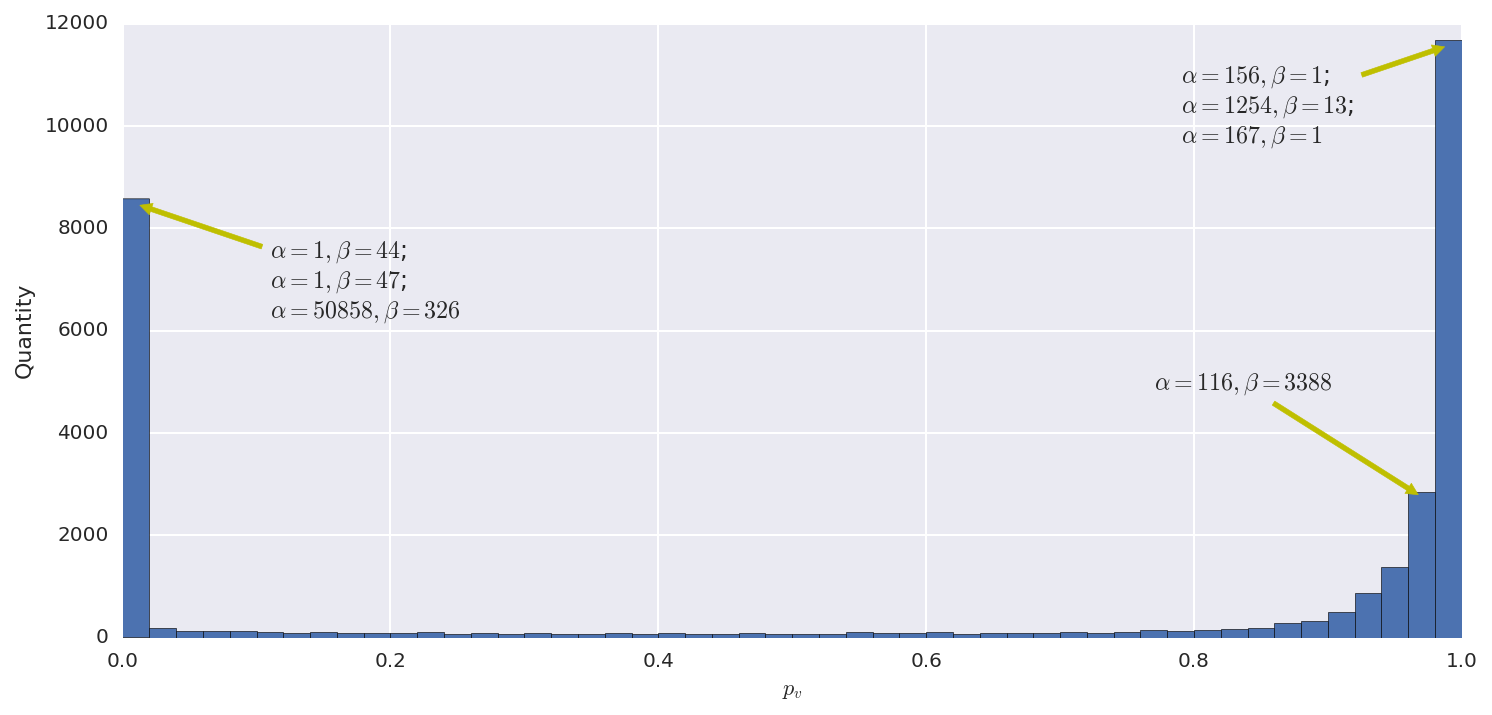
\includegraphics[width=\textwidth]{figures/bayes/hist_time.png}
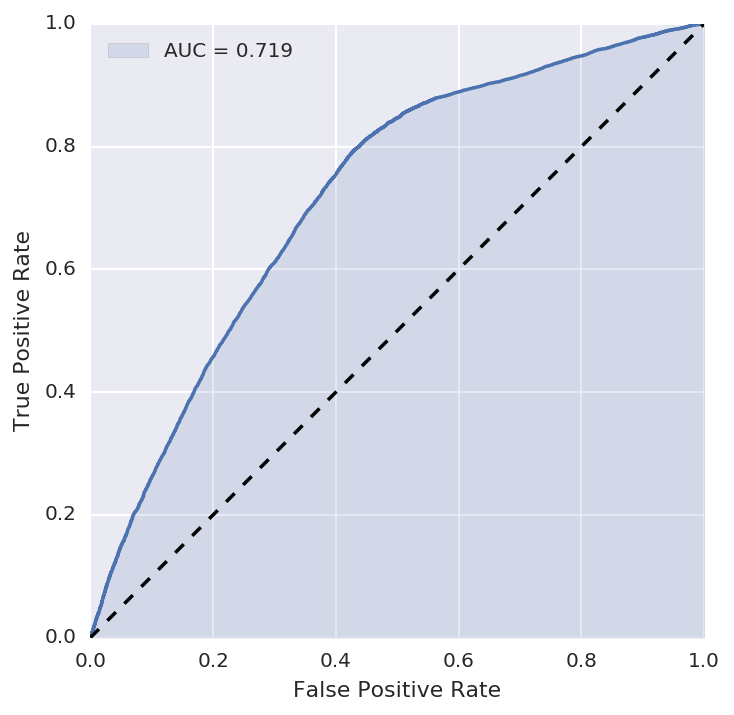
\includegraphics[width=.49\textwidth]{figures/bayes/roc_time.png}
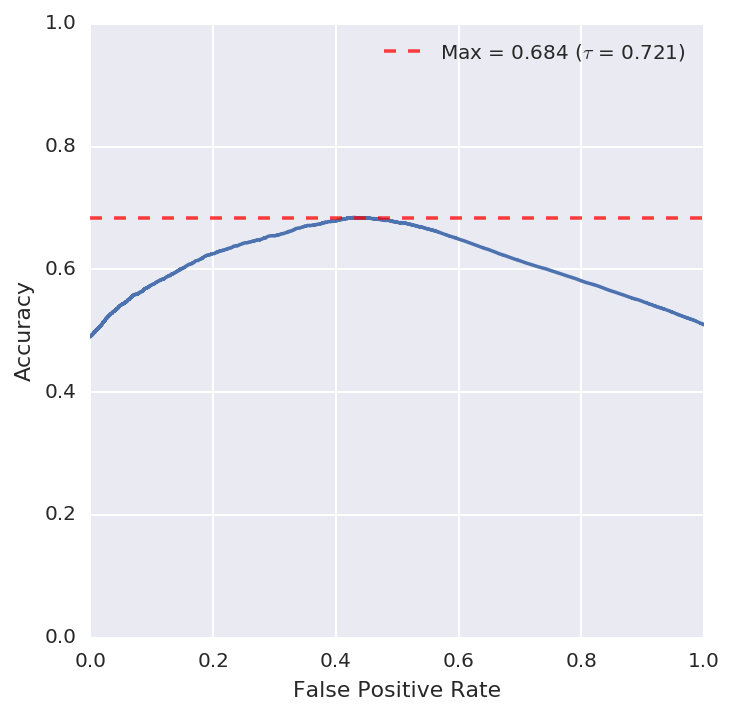
\includegraphics[width=.49\textwidth]{figures/bayes/accuracy_time.png}
\end{center}

When $\varpi = \etime$ and the data is analyzed using $\Upsilon^{\calls}$ as \emph{Testing Set}, there are two big clusters of data at the edges. The reason for these is that, as shown by Figure~\ref{fig:timeheatmap}, the majority of users only call either \emph{High Income} or \emph{Low Income} users. For completeness sake, this test is run again in Section~\ref{fig:time_infer_positive} only for the subset $\hat{\Upsilon}^{\calls} \subseteq \Upsilon^{\calls}$ which have at least one call to users of each income category; however, while this makes the histogram more equitative taking out the users with SMS to both categories (whose users tend to be in that same category) makes all the metrics lower.

The \emph{Area Under the Curve} of this inference mechanism is $\AUC = 0.719$, which is lower than the one for the calls in Section~\ref{subsec:call_infer}. The \emph{Accuracy Curve} is unsurprisingly similar to that one, and even the \emph{Accuracy} at $\tau = 0.721$ is the same. This is probably a result of using the same dataset as that section, and the fact that there is an obvious correlation between total talking time and total calls, shown in Figure~\ref{fig:call_time}.

That value of $\tau$ also results in a predictor where $\Accuracy = 0.684$, $\FPR = 123$, $\Precision = 123$, $\Recall = 123$, $F_1 = 123$, and $F_4 = 123$. \todo{Fill these values.}

\subsubsection{Inferring by SMS}
\label{subsec:sms_infer}

\begin{center}
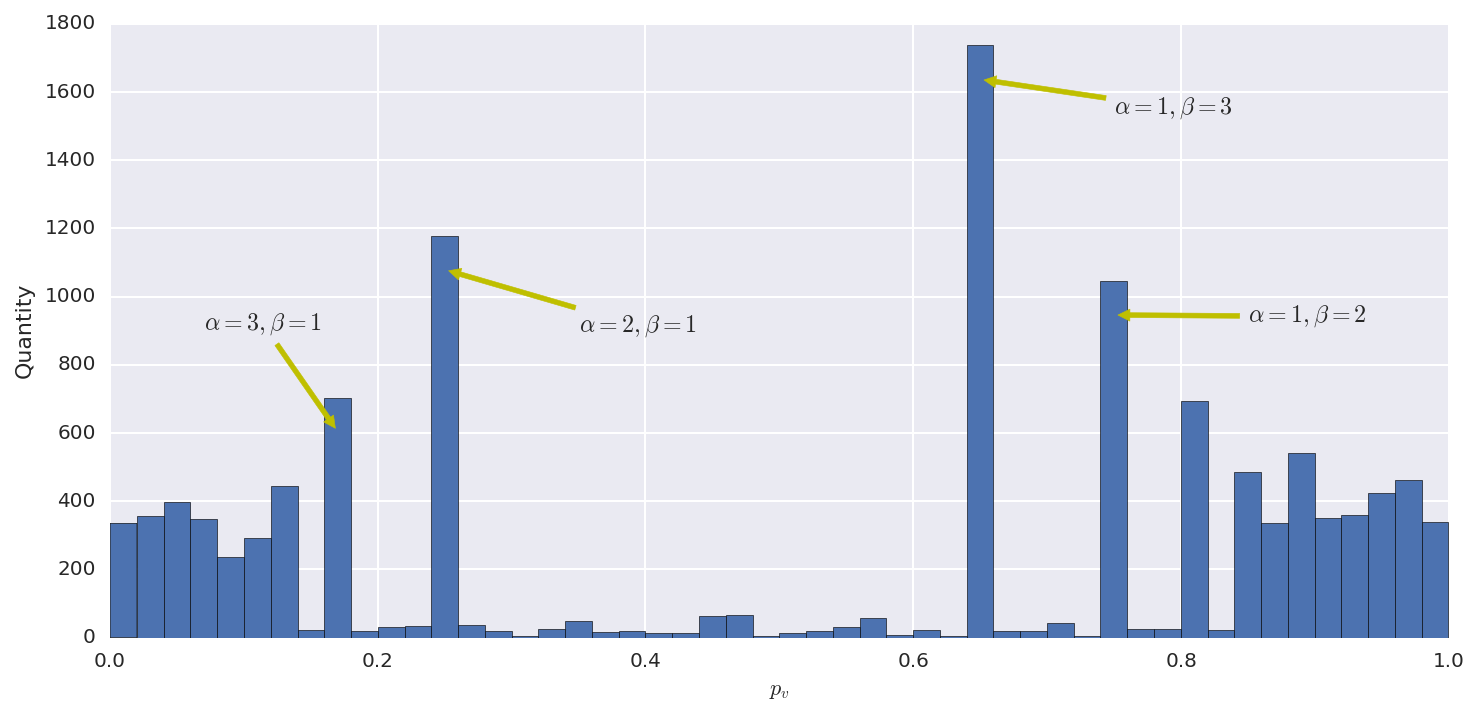
\includegraphics[width=\textwidth]{figures/bayes/hist_sms.png}
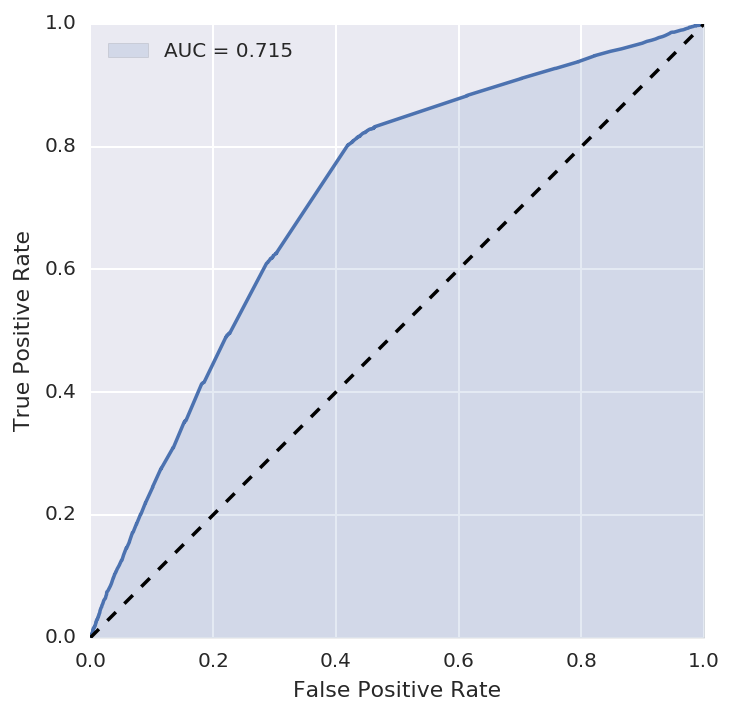
\includegraphics[width=.49\textwidth]{figures/bayes/roc_sms.png}
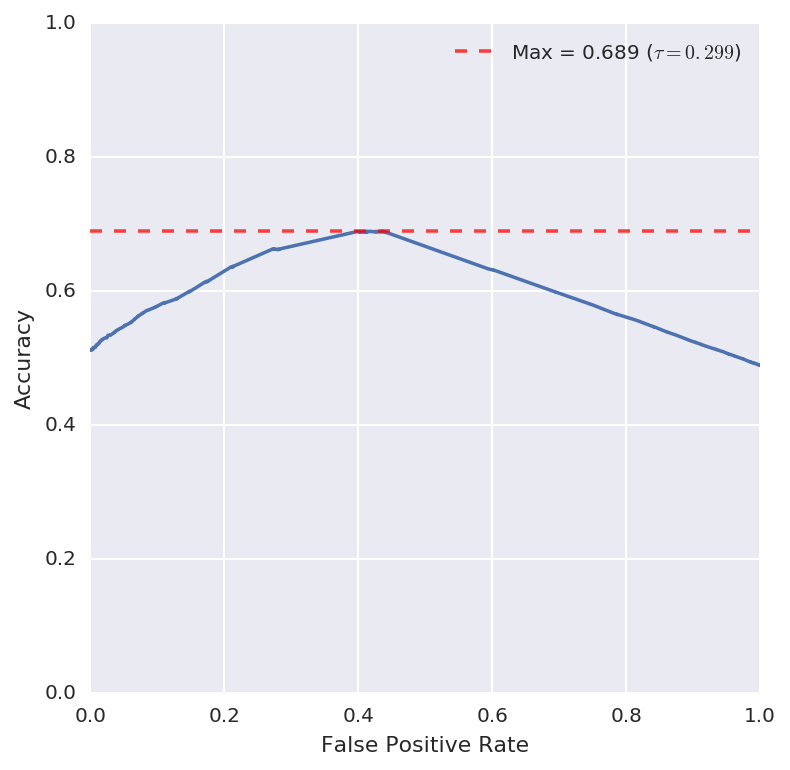
\includegraphics[width=.49\textwidth]{figures/bayes/accuracy_sms.png}
\end{center}

Since the total amount of SMS is much lower than the amount of calls, the peaks of the result of the \emph{Inverse Cumulative Functions} of the \emph{Beta Distribution} applied on $\Upsilon^{\sms}$ that happen with the majority of users that have few of both are located closer to the center than in Section~\ref{subsec:call_infer} and Section~\ref{subsec:time_infer}. This makes some interesting cases if $\varpi = \sms$ is chosen, since the distribution is different than in the other cases.

In particular, this gives an $\AUC = 0.715$, which is lower than both in the case of \emph{Calls} and \emph{Time}. Interesingly, the maximum \emph{Accuracy} at $\tau = 0.224$ is slightly higher than both of the other cases; this is probably a side-effect of the fact that $\left| \Upsilon^{\sms} \right| < \left| \Upsilon^{\calls} \right|$.

Additionally, $\FPR = 123$, $\Precision = 123$, $\Recall = 123$, $F_1 = 123$, and $F_4 = 123$. \todo{Fill these values.}

\subsubsection{Inferring by Contacts}
\label{subsec:contacts_infer}

\begin{center}
\includegraphics[width=\textwidth]{figures/bayes/hist_contacts.png}
\includegraphics[width=.49\textwidth]{figures/bayes/roc_contacts.png}
\includegraphics[width=.49\textwidth]{figures/bayes/accuracy_contacts.png}
\end{center}

When $\varpi = \contacts$ it's possible to get a pattern similar to the one shown in Section~\ref{subsec:sms_infer} when $\varpi = \sms$, where the majority of users have relatively few contacts and the peaks in the histogram. Additionally, since the total amount of contacts is logarithmically distributed (as shown in Figure~\ref{fig:contact_distribution}), and people with \emph{High Income} tend to have more contacts in general, there peaks are clustered in areas with low $p_v$ (where the majority of calls are made to \emph{Low Income} users), near the middle (where the calls are mostly equally distributed), but not at high $p_v$; this last section would belong to the few users with many calls to \emph{High Income} users.

Using this method it's possible to find that $\AUC = 0.742$, which is higher than all the other methods presented in Section~\ref{subsec:algorithm_performance}. Additionally, when selecting $\tau = 0.224$, $\Accuracy = 0.691$ which is higher than the maximum \emph{Accuracy} in all other methods. These metrics, combined with the fact that $\Upsilon$ contains every user in the \emph{Testing Set}, result in the fact that $\varpi = \contacts$ is uambiguously the best way to classify the data for the algorithm. Additionally, $\FPR = 123$, $\Precision = 123$, $\Recall = 123$, $F_1 = 123$, and $F_4 = 123$.

\subsection{Algorithm Performance of Users with at least 3 Contacts}

The algorithm tends to be a better predictor of the \emph{Socioeconomic Level} for users with high amount of information on the graph $G$, namely that the amount of users in their neighbourhood that also belong to $B$ is big.

In this section, we run the \emph{Bayesian Algorithm} for the subset of the users presented in Equation~\ref{eq:3contacts}, which restrict the users in the \emph{Testing Set} to only those who have at least 3 contacts. This would allow us to have better metrics in the dataset, at the expense of a much smaller Universe of users for which the algorithm could be applied. Additionally, Table~\ref{tab:3contacts} shows the sizes of the \emph{Testing Sets} used in a manner similar to Table~\ref{tab:partition_numbers}.

\begin{equation}
\label{eq:3contacts}
\begin{gathered}
I = \left\{ \upsilon \in \Upsilon \mid \contacts^{high}_{\upsilon} + \contacts^{\low}_{\upsilon} > 3 \right\} \\
I^{\calls} = \Upsilon^{\calls} \cap I
\end{gathered}
\end{equation}

\begin{table}
\centering
\begin{tabular}{l r r r c}
\toprule
Set & Total Size & High Income & Low Income & Ratio \\
\midrule
$I$ & \num{7932} & \num{4637} & \num{3295} & \num{0.258} \\
$I^{\calls}$ & \num{7910} & \num{4627} & \num{3283} & \num{0.214} \\
\bottomrule
\end{tabular}
\caption{Amount of users in the \emph{Testing Set} after trimming it several to only have users with at least 3 contacts.}
\label{tab:3contacts}
\end{table}

The same procedure applied in Section~\ref{subsec:calls_infer} and Section~\ref{subsec:contacts_infer} will be applied to this data.

\subsubsection{Inferring by Calls on Users with at least 3 Contacts}

\begin{center}
\includegraphics[width=\textwidth]{figures/bayes/3contacts/hist_calls.png}
\includegraphics[width=.49\textwidth]{figures/bayes/3contacts/roc_calls.png}
\includegraphics[width=.49\textwidth]{figures/bayes/3contacts/accuracy_calls.png}
\end{center}

Using $I^{\calls} \subseteq \Upsilon^{\calls}$ and $\varpi = \calls$ results in a predictor where both the \emph{Area Under the Curve} and the \emph{Accuracy} are higher than in all predictors that use every possible user. However, this data predicts less users and is strictly worse than the one predicting by Contacts presented in the following section.

\subsubsection{Inferring by Degree on Users with at least 3 Contacts}

\begin{center}
\includegraphics[width=\textwidth]{figures/bayes/3contacts/hist_contacts.png}
\includegraphics[width=.49\textwidth]{figures/bayes/3contacts/roc_contacts.png}
\includegraphics[width=.49\textwidth]{figures/bayes/3contacts/accuracy_contacts.png}
\end{center}

This dataset results in the best possible predictor for a reasonable subset of the users. Both the \emph{Area Under the Curve} and the \emph{Accuracy} are higher than for all other predictors: $\AUC = 0.829$, $\Accuracy = 0.766$, $\FPR = 123$, $\TPR = 123$, $\Precision = 123$, $\Recall = 123$, $F_1 = 123$, and $F_4 = 123$.

All of those values are considerably better than any other predictor in this page at the cost of using only a small subset of the possible users. This is interesing as it's exactly the same subset as the one used in~\cite{fixmanasonam2016}, and it scores significantly higher in all the metrics.


\bibliography{../Tesis/bibliography/sna}{}

\end{document}
